%% LyX 2.3.6 created this file.  For more info, see http://www.lyx.org/.
%% Do not edit unless you really know what you are doing.
\documentclass[english]{article}
\usepackage[T1]{fontenc}
\usepackage[latin9]{inputenc}
\usepackage{url}
\usepackage{graphicx}

\makeatletter

%%%%%%%%%%%%%%%%%%%%%%%%%%%%%% LyX specific LaTeX commands.
%% Because html converters don't know tabularnewline
\providecommand{\tabularnewline}{\\}

\makeatother

\usepackage{babel}
\begin{document}
\title{NeuralMinimizer, a novel method for global optimization that incorporates
machine learning}
\author{Ioannis G. Tsoulos$^{(1)}$\thanks{Corresponding author. Email: itsoulos@uoi.gr},
Alexandros Tzallas$^{(1)}$, \\
Evangelos Karvounis$^{(1)}$, Dimitrios Tsalikakis$^{(2)}$}
\date{$^{(1)}$Department of Informatics and Telecommunications, University
of Ioannina, 47100 Arta, Greece \\
$^{(2)}$University of Western Macedonia, Department of Engineering
Informatics and Telecommunications, Greece}
\maketitle
\begin{abstract}
The problem of finding the global minimum of multidimensional functions
is often applied to a wide range of problems. An innovative technique
for finding the global minimum is proposed in this paper. In this
technique, an estimation of the objective function is constructed
using an RBF network. The network constantly updates the estimation
for the objective function with information it gathers from performing
local minimizations. In addition, the proposed technique uses as a
termination criterion a widely used criterion from the relevant literature
which in fact evaluates it after each execution of the local minimization.
The proposed technique was applied to a number of well-known problems
from the relevant literature, and the comparative results with respect
to modern global minimization techniques are extremely promising.
\end{abstract}

\section{Introduction }

An innovative method for finding the global minimum of multidimensional
functions is presented here. The functions considered are continuous
and differentiable function and defined as $f:S\rightarrow R,S\subset R^{n}$.
The problem of locating the global optimum is usually formulated as:
\begin{equation}
x^{*}=\mbox{arg}\min_{x\in S}f(x)\label{eq:eq1}
\end{equation}
with $S$: 
\[
S=\left[a_{1},b_{1}\right]\otimes\left[a_{2},b_{2}\right]\otimes\ldots\left[a_{n},b_{n}\right]
\]
A variety of problems in the physical world can be represented as
global minimum problems, such as problems from physics \cite{go_physics1,go_physics2,go_physics3},
chemistry \cite{go_chemistry1,go_chemistry2,go_chemistry3}, economics
\cite{go_econ1,go_econ2}, medicine \cite{go_med1,go_med2} etc. During
the past years many methods, especially stochastic one, have been
proposed to tackle the problem of equation \ref{eq:eq1}, such as
Controlled Random Search methods \cite{crs1,crs2,crs3} , Simulated
Annealing methods \cite{simann_major,simann1,simann2}, Differential
Evolution methods \cite{diffe1,diffe2}, Particle Swarm Optimization
(PSO) methods \cite{pso_major,pso1,pso2}, Ant Colony Optimization
\cite{aco1,aco2}, Genetic algorithms \cite{ga1,ga2,ga3} etc. A systematic
review of global optimization methods can also be found in the work
of Floudas et al \cite{FloudasReview}. In addition, during the last
few years, a variety of work has been proposed on combinations and
modifications to some global optimization methods to more efficiently
find the global minimum, such as methods that combine PSO with other
methods \cite{pso_hybrid1,pso_hybrid2,pso_hybrid3}, methods aimed
to discover all the local minima of functions \cite{tmlsl,Salhi,minfinder},
new stopping rules to efficiently terminate the global optimization
techniques \cite{msstop1,msstop2,msstop3} etc. Also, due to the massive
use of parallel processing techniques, several methods have been proposed
that take full advantage of parallel processing, such as parallel
techniques \cite{parallel-pso,parallel-multistart,parallel-doublepop},
methods that utilize the GPU architectures \cite{msgpu1,msgpu2} etc.

In this paper, a new multi-start method is proposed that uses a machine
learning model, which is trained in parallel with the evolution of
the optimization process. Although multistart methods are considered
the basis for more modern optimization techniques, they have been
successfully used in several problems such as the Traveling Salesman
Problem (TSP)\textbf{ }\cite{multistart-tsp1,multistart_tsp2,multistart_tsp3},
the maximum clique problem \cite{ms_clique1,ms_clique2}, the vehicle
routing problem \cite{multistart-vehicle1,multistart-vehicle2}, scheduling
problems \cite{ms_schedule1,ms_schedule2} etc. In the new technique,
a Radial Basis Function (RBF) network \cite{rbf_main1} is used to
construct an approximation of the objective function. This construction
is carried out in parallel with the execution of the optimization.
A limited number of samples from the objective function and the local
minima discovered during the optimization are used to construct the
approximation function. During the execution of the method, the samples
needed to start local minimizers are taken from the approximation
function that is constructed by the neural network. The RBF network
was used as an approximation tool as it has been successfully used
in a wide range of problems in the field of artificial intelligence
\cite{rbf_face,rbf_function1,rbf_function2,rbf_image} and its training
procedure is very fast, if compared to artificial neural networks
for example. In addition, for more efficient termination of the method,
a termination method proposed by Tsoulos is used \cite{Tsoulos1},
but this termination method is applied after each execution of the
local minimization procedure. The proposed technique was applied to
a series of problems from the relevant literature and the results
are extremely promising even compared to established global optimization
techniques.

The rest of this article is organized as follows: in section \ref{sec:Method-Description}
the description of the proposed method is provided, in section \ref{sec:Experiments}
the used experimental functions as well as the experimental results
and comparisons are listed and finally in section \ref{sec:Conclusions}
some conclusions and final thoughts are given.

\section{Method Description \label{sec:Method-Description}}

The proposed technique generates an estimation of the objective function
during the optimization using an RBF network. This estimation is initially
generated from some samples from the objective function and gradually
local minima that will have been discovered during the optimization
are added to it. In this way, the estimation of the objective function
will be continuously improved to approximate the true function as
much as possible. At every iteration, several samples are then taken
from the estimated function and sorted in ascending order. Those with
the lowest value will be starting points of the local minimization
method. The local optimization method used here is a BFGS variant
of Powell \cite{powell}. This process has the effect of drastically
reducing the total number of function calls that are made and, at
the same time, the points used as initiators of the local minimization
technique approach the global minimum of the objective function. Also,
the proposed method checks the termination rule after the application
of every local search method. That way, if the absolute minimum has
already been discovered with some certainty, no more function calls
will be wasted finding it.

In the following subsections, the training procedure of RBF networks
as well as the proposed method are fully described.

\subsection{Rbf preliminaries}

An RBF network can be defined as:\textbf{
\begin{equation}
N\left(\overrightarrow{x}\right)=\sum_{i=1}^{k}w_{i}\phi\left(\left\Vert \overrightarrow{x}-\overrightarrow{c_{i}}\right\Vert \right)\label{eq:firstrbf}
\end{equation}
}Where 
\begin{enumerate}
\item The vector $\overrightarrow{x}$ is called the input pattern to the
equation. 
\item The vectors $\overrightarrow{c_{i}},\ i=1,..,k$ are called the center
vectors.
\item The vector $\overrightarrow{w}$ stands for the the output weight
of the RBF network.
\end{enumerate}
In most cases the function $\phi(x)$ is a Gaussian function:\textbf{
\begin{equation}
\phi(x)=\exp\left(-\frac{\left(x-c\right)^{2}}{\sigma^{2}}\right)
\end{equation}
}A plot for this function with $c=0,\ \sigma=1$ is shown in Figure
\ref{fig:A-plot-for}. The training error for the RBF network on a
set $T=\left\{ \left(x_{1},y_{1}\right),\left(x_{2},y_{2}\right),\ldots,\left(x_{M},y_{M}\right)\right\} $
points is estimated as
\begin{equation}
E\left(N\left(\overrightarrow{x}\right)\right)=\sum_{i=1}^{M}\left(N\left(x_{i}\right)-y_{i}\right)^{2}\label{eq:rbf_error}
\end{equation}
In most approaches, the equation \ref{eq:rbf_error} is minimized
with respect to the parameters of the RBF network using a two phase
procedure:
\begin{enumerate}
\item During the first phase, the $k$ centers and the corresponding variances
are calculated using the K-Means algorithm \cite{kmeans}.
\item During the second phase, the weights $\overrightarrow{w}=\left(w_{1},w_{2},\ldots,w_{k}\right)$
are calculated by solving a linear system of equations with the following
procedure:
\begin{enumerate}
\item \textbf{Set} \textbf{$W=w_{kj}$}
\item \textbf{Set} \textbf{$\Phi=\phi_{j}\left(x_{i}\right)$}
\item \textbf{Set $T=\left\{ t_{i}=f\left(x_{i}\right),i=1,..,M\right\} $. }
\item The system to be solved is identified as:\textbf{ 
\begin{equation}
\Phi^{T}\left(T-\Phi W^{T}\right)=0
\end{equation}
}With solution:\textbf{
\begin{equation}
W^{T}=\left(\Phi^{T}\Phi\right)^{-1}\Phi^{T}T=\Phi^{\dagger}T\label{eq:eqoutput}
\end{equation}
}
\end{enumerate}
\end{enumerate}
\begin{figure}
\caption{A plot for the Gaussian function.\label{fig:A-plot-for}}

\centering{}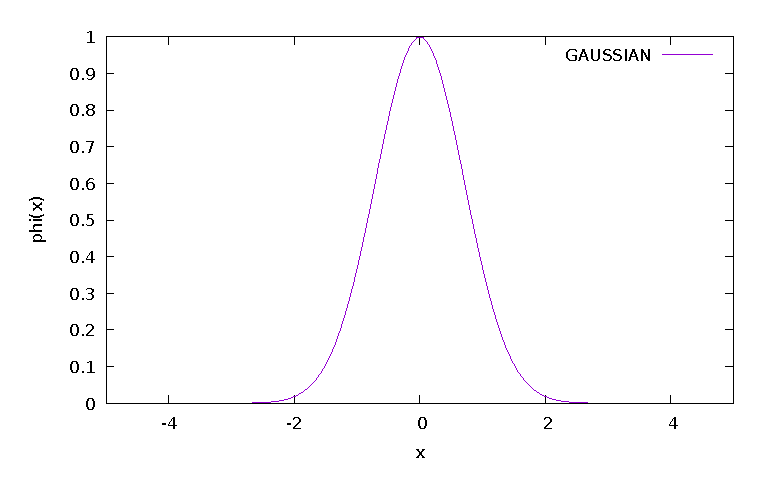
\includegraphics[scale=0.7]{gaussian}
\end{figure}


\subsection{The main algorithm}

The main steps of the proposed algorithm have as follows:
\begin{enumerate}
\item \textbf{Initialization} step.
\begin{enumerate}
\item \textbf{Set} $k$ the number of weights in RBF network.
\item \textbf{Set} $N_{S}$ the initial samples that will be taken from
the function $f(x)$.
\item \textbf{Set} $N_{T}$ the number of samples, that will used in every
iteration as starting points for the local optimization procedure.
\item Set $N_{R}$ the number of samples that will be drawn from the RBF
network at every iteration with $N_{R}>N_{T}$
\item \textbf{Set} $N_{G}$ the maximum number of allowed iterations.
\item \textbf{Set} Iter=0, the iteration number.
\item \textbf{Set} $\left(x^{*},y^{*}\right)$ as the global minimum. Initially
$y^{*}=\infty$
\end{enumerate}
\item \textbf{Creation }Step.
\begin{enumerate}
\item \textbf{Set} $T=\emptyset$, the training set for the RBF network.
\item \textbf{For} $i=1,..,N_{S}$ do
\begin{enumerate}
\item \textbf{Take} a new sample $x_{i}\in S$
\item \textbf{Calculate} $y_{i}=f\left(x_{i}\right)$
\item $T=T\cup\left(x_{i},y_{i}\right)$
\end{enumerate}
\item \textbf{EndFor}
\item \textbf{Train} the RBF network on the training set $T$.
\end{enumerate}
\item \textbf{Sampling }Step
\begin{enumerate}
\item \textbf{Set} $T_{R}=\emptyset$
\item \textbf{For} $i=1,..,N_{R}$ \textbf{do}
\begin{enumerate}
\item \textbf{Take} a random sample $\left(x_{i},y_{i}\right)$ from the
RBF network.
\item \textbf{Set} $T_{R}=T_{R}\cup\left(x_{i,}y_{i}\right)$
\end{enumerate}
\item \textbf{EndFor}
\item \textbf{Sort} $T_{R}$ according to the y values in ascending order.
\end{enumerate}
\item \textbf{Optimization} Step.
\begin{enumerate}
\item \textbf{For} $i=1,..,N_{T}$ do
\begin{enumerate}
\item \textbf{Take} the next sample $\left(x_{i},y_{i}\right)$ from $T_{R}$.
\item $y_{i}=\mbox{LS}\left(x_{i}\right)$. Where LS(x) is a predefined
local search method.
\item $T=T\cup\left(x_{i},y_{i}\right)$, this step updates the training
set of the RBF network.
\item \textbf{Train} the RBF network on set $T$.
\item \textbf{If} $y_{i}\le y^{*}$ then $x^{*}=x_{i},y^{*}=y_{i}$
\item \textbf{Check} the termination rule as suggested in \cite{Tsoulos1}.
If it holds report $\left(x^{*},y^{*}\right)$ as the located global
minimum and terminate.
\end{enumerate}
\item \textbf{EndFor}
\end{enumerate}
\item \textbf{Set} iter=iter+1
\item \textbf{Goto} to Sampling step.
\end{enumerate}

\section{Experiments \label{sec:Experiments}}

\subsection{Test functions }

To estimate the efficiency of the new technique a number of functions
from the relevant literature were used \cite{Ali1,Floudas1}. These
functions are provided in the following.
\begin{itemize}
\item \textbf{\emph{Bent Cigar function}}\emph{ }The function is 
\[
f(x)=x_{1}^{2}+10^{6}\sum_{i=2}^{n}x_{i}^{2}
\]
 with the global minimum $f\left(x^{*}\right)=0$. For the conducted
experiments the value $n=10$ was used.
\item \textbf{Bf1} function. The function Bohachevsky 1 is given by the
equation
\end{itemize}
\[
f(x)=x_{1}^{2}+2x_{2}^{2}-\frac{3}{10}\cos\left(3\pi x_{1}\right)-\frac{4}{10}\cos\left(4\pi x_{2}\right)+\frac{7}{10}
\]
with $x\in[-100,100]^{2}$. 
\begin{itemize}
\item \textbf{Bf2} function. The function Bohachevsky 2 is given by the
equation 
\[
f(x)=x_{1}^{2}+2x_{2}^{2}-\frac{3}{10}\cos\left(3\pi x_{1}\right)\cos\left(4\pi x_{2}\right)+\frac{3}{10}
\]
with $x\in[-50,50]^{2}$. 
\item \textbf{Branin} function. The function is defined by $f(x)=\left(x_{2}-\frac{5.1}{4\pi^{2}}x_{1}^{2}+\frac{5}{\pi}x_{1}-6\right)^{2}+10\left(1-\frac{1}{8\pi}\right)\cos(x_{1})+10$
with $-5\le x_{1}\le10,\ 0\le x_{2}\le15$. The value of global minimum
is 0.397887.with $x\in[-10,10]^{2}$. 
\item \textbf{CM} function. The Cosine Mixture function is given by the
equation 
\[
f(x)=\sum_{i=1}^{n}x_{i}^{2}-\frac{1}{10}\sum_{i=1}^{n}\cos\left(5\pi x_{i}\right)
\]
with $x\in[-1,1]^{n}$. For the conducted experiments the value $n=4$
was used.
\item \textbf{Camel} function. The function is given by 
\[
f(x)=4x_{1}^{2}-2.1x_{1}^{4}+\frac{1}{3}x_{1}^{6}+x_{1}x_{2}-4x_{2}^{2}+4x_{2}^{4},\quad x\in[-5,5]^{2}
\]
The global minimum has the value of $f\left(x^{*}\right)=-1.0316$
\item \textbf{Discus function}\emph{ }The function is defined as 
\[
f(x)=10^{6}x_{1}^{2}+\sum_{i=2}^{n}x_{i}^{2}
\]
 with global minimum $f\left(x^{*}\right)=0.$ For the conducted experiments
the value $n=10$ was used.
\item \textbf{Easom} function The function is given by the equation 
\[
f(x)=-\cos\left(x_{1}\right)\cos\left(x_{2}\right)\exp\left(\left(x_{2}-\pi\right)^{2}-\left(x_{1}-\pi\right)^{2}\right)
\]
with $x\in[-100,100]^{2}$ and global minimum -1.0
\item \textbf{Exponential} function. The function is given by 
\[
f(x)=-\exp\left(-0.5\sum_{i=1}^{n}x_{i}^{2}\right),\quad-1\le x_{i}\le1
\]
The global minimum is located at $x^{*}=(0,0,...,0)$ with value $-1$.
In our experiments we used this function with $n=4,16,64$ and the
corresponding functions are denoted by the labels EXP4, EXP16, EXP64.
\item \textbf{Griewank10} function. The function is given by the equation
\[
f(x)=\sum_{i=1}^{n}\frac{x_{i}^{2}}{4000}-\prod_{i=1}^{n}\cos\left(\frac{x_{i}}{\sqrt{i}}\right)+1
\]
with $n=10$.
\item \textbf{Hansen} function. $f(x)=\sum_{i=1}^{5}i\cos\left[(i-1)x_{1}+i\right]\sum_{j=1}^{5}j\cos\left[(j+1)x_{2}+j\right]$,
$x\in[-10,10]^{2}$ . The global minimum of the function is -176.541793.
\item \textbf{Hartman 3} function. The function is given by
\[
f(x)=-\sum_{i=1}^{4}c_{i}\exp\left(-\sum_{j=1}^{3}a_{ij}\left(x_{j}-p_{ij}\right)^{2}\right)
\]
with $x\in[0,1]^{3}$ and $a=\left(\begin{array}{ccc}
3 & 10 & 30\\
0.1 & 10 & 35\\
3 & 10 & 30\\
0.1 & 10 & 35
\end{array}\right),\ c=\left(\begin{array}{c}
1\\
1.2\\
3\\
3.2
\end{array}\right)$ and
\[
p=\left(\begin{array}{ccc}
0.3689 & 0.117 & 0.2673\\
0.4699 & 0.4387 & 0.747\\
0.1091 & 0.8732 & 0.5547\\
0.03815 & 0.5743 & 0.8828
\end{array}\right)
\]
The value of global minimum is -3.862782.
\item \textbf{Hartman 6} function.
\[
f(x)=-\sum_{i=1}^{4}c_{i}\exp\left(-\sum_{j=1}^{6}a_{ij}\left(x_{j}-p_{ij}\right)^{2}\right)
\]
with $x\in[0,1]^{6}$ and $a=\left(\begin{array}{cccccc}
10 & 3 & 17 & 3.5 & 1.7 & 8\\
0.05 & 10 & 17 & 0.1 & 8 & 14\\
3 & 3.5 & 1.7 & 10 & 17 & 8\\
17 & 8 & 0.05 & 10 & 0.1 & 14
\end{array}\right),\ c=\left(\begin{array}{c}
1\\
1.2\\
3\\
3.2
\end{array}\right)$ and
\[
p=\left(\begin{array}{cccccc}
0.1312 & 0.1696 & 0.5569 & 0.0124 & 0.8283 & 0.5886\\
0.2329 & 0.4135 & 0.8307 & 0.3736 & 0.1004 & 0.9991\\
0.2348 & 0.1451 & 0.3522 & 0.2883 & 0.3047 & 0.6650\\
0.4047 & 0.8828 & 0.8732 & 0.5743 & 0.1091 & 0.0381
\end{array}\right)
\]
the value of global minimum is -3.322368.
\item \textbf{High Conditioned Elliptic} function, defined as 
\[
f(x)=\sum_{i=1}^{n}\left(10^{6}\right)^{\frac{i-1}{n-1}}x_{i}^{2}
\]
with global minimum $f\left(x^{*}\right)=0$ and the value $n=10$
was used in the conducted experiments
\item \textbf{Potential} function. The molecular conformation corresponding
to the global minimum of the energy of N atoms interacting via the
Lennard-Jones potential\cite{Jones} is used as a test case here.
The function to be minimized is given by:
\begin{equation}
V_{LJ}(r)=4\epsilon\left[\left(\frac{\sigma}{r}\right)^{12}-\left(\frac{\sigma}{r}\right)^{6}\right]\label{eq:potential}
\end{equation}
In the current experiments two different cases were studied: $N=3,\ 5$
\item \textbf{Rastrigin} function. The function is given by 
\[
f(x)=x_{1}^{2}+x_{2}^{2}-\cos(18x_{1})-\cos(18x_{2}),\quad x\in[-1,1]^{2}
\]
\item \textbf{Shekel 7} function.
\end{itemize}
\[
f(x)=-\sum_{i=1}^{7}\frac{1}{(x-a_{i})(x-a_{i})^{T}+c_{i}}
\]

with $x\in[0,10]^{4}$ and $a=\left(\begin{array}{cccc}
4 & 4 & 4 & 4\\
1 & 1 & 1 & 1\\
8 & 8 & 8 & 8\\
6 & 6 & 6 & 6\\
3 & 7 & 3 & 7\\
2 & 9 & 2 & 9\\
5 & 3 & 5 & 3
\end{array}\right),\ c=\left(\begin{array}{c}
0.1\\
0.2\\
0.2\\
0.4\\
0.4\\
0.6\\
0.3
\end{array}\right)$. 
\begin{itemize}
\item \textbf{Shekel 5 }function.
\end{itemize}
\[
f(x)=-\sum_{i=1}^{5}\frac{1}{(x-a_{i})(x-a_{i})^{T}+c_{i}}
\]
 

with $x\in[0,10]^{4}$ and $a=\left(\begin{array}{cccc}
4 & 4 & 4 & 4\\
1 & 1 & 1 & 1\\
8 & 8 & 8 & 8\\
6 & 6 & 6 & 6\\
3 & 7 & 3 & 7
\end{array}\right),\ c=\left(\begin{array}{c}
0.1\\
0.2\\
0.2\\
0.4\\
0.4
\end{array}\right)$. 
\begin{itemize}
\item \textbf{Shekel 10} function.
\end{itemize}
\[
f(x)=-\sum_{i=1}^{10}\frac{1}{(x-a_{i})(x-a_{i})^{T}+c_{i}}
\]
 

with $x\in[0,10]^{4}$ and $a=\left(\begin{array}{cccc}
4 & 4 & 4 & 4\\
1 & 1 & 1 & 1\\
8 & 8 & 8 & 8\\
6 & 6 & 6 & 6\\
3 & 7 & 3 & 7\\
2 & 9 & 2 & 9\\
5 & 5 & 3 & 3\\
8 & 1 & 8 & 1\\
6 & 2 & 6 & 2\\
7 & 3.6 & 7 & 3.6
\end{array}\right),\ c=\left(\begin{array}{c}
0.1\\
0.2\\
0.2\\
0.4\\
0.4\\
0.6\\
0.3\\
0.7\\
0.5\\
0.6
\end{array}\right)$. 
\begin{itemize}
\item \textbf{Sinusoidal} function. The function is given by 
\[
f(x)=-\left(2.5\prod_{i=1}^{n}\sin\left(x_{i}-z\right)+\prod_{i=1}^{n}\sin\left(5\left(x_{i}-z\right)\right)\right),\quad0\le x_{i}\le\pi.
\]
The global minimum is located at $x^{*}=(2.09435,2.09435,...,2.09435)$
with $f\left(x^{*}\right)=-3.5$. For the conducted experiments the
cases of $n=4,8$ and $z=\frac{\pi}{6}$ were studied.
\item \textbf{Test2N} function. This function is given by the equation 
\[
f(x)=\frac{1}{2}\sum_{i=1}^{n}x_{i}^{4}-16x_{i}^{2}+5x_{i},\quad x_{i}\in[-5,5].
\]
The function has $2^{n}$ in the specified range and in our experiments
we used $n=4,5,6,7$. 
\item \textbf{Test30N} function. This function is given by 
\[
f(x)=\frac{1}{10}\sin^{2}\left(3\pi x_{1}\right)\sum_{i=2}^{n-1}\left(\left(x_{i}-1\right)^{2}\left(1+\sin^{2}\left(3\pi x_{i+1}\right)\right)\right)+\left(x_{n}-1\right)^{2}\left(1+\sin^{2}\left(2\pi x_{n}\right)\right)
\]
with $x\in[-10,10]$. The function has $30^{n}$ local minima in the
specified range and we used $n=3,4$ in the conducted experiments.
\end{itemize}

\subsection{Experimental results}

The proposed technique was tested on the previously presented test
functions and the results produced were compared with those given
by a simple genetic algorithm or a PSO method. In order to have fairness
in the comparison of the results, both in the case of genetic algorithms
and in the case of the PSO method, the same local minimization method
has been used as that of the proposed method. In addition, the number
of chromosomes in the genetic algorithm and the number of particles
in the PSO method are identical to the parameter $N_{T}$ of the proposed
procedure. The values for the used parameters are listed in Table
\ref{tab:Experimental-settings.}. The conducted experiments were
executed 30 times for each test function and averages were taken.
In each execution, different seed for the random generator was used.
The proposed method is implemented as the method with the name \emph{NeuralMinimizer}
in the \emph{OPTIMUS} global optimization environment, which is freely
available from \url{https://github.com/itsoulos/OPTIMUS}. All the
experiments were conducted on an AMD Ryzen 5950X with 128GB of RAM
and the Debian Linux operating system. 

The experimental results from the application of the proposed method
and the Genetic algorithm and the PSO method are shown in Table \ref{tab:Comparison}.
The number show in the cells denote average function calls. The fraction
in parentheses represents the fraction of executions where the global
optimum was successfully found. When this number is absent, then the
global minimum is computed for every execution (100\% success). At
the end of the table, an additional row named AVERAGE indicates the
total number of function calls and the average success rate in locating
the global minimum. In the experimental results, the superiority of
the proposed technique over the other two methods in terms of the
number of function calls is clear. The proposed technique requires
an average of 90\% fewer function calls than the other methods. In
addition, the proposed technique appears to be more efficient than
the other two as it finds more times on average the global minimum
of most test functions in the experiments.

In addition, the table \ref{tab:kexperiments} presents the experimental
results for the proposed method and for various values of the parameter
$N_{S}$. As can be seen, the increase in this parameter does not
cause a large increase in the total number of function calls, while
at the same time it improves to some extent the ability of the proposed
technique to find the global minimum.

\begin{table}
\caption{Experimental settings.\label{tab:Experimental-settings.}}

\centering{}%
\begin{tabular}{|c|c|c|}
\hline 
PARAMETER & MEANING & VALUE\tabularnewline
\hline 
\hline 
$k$ & Number of weights & 10\tabularnewline
\hline 
$N_{S}$ & Start samples & 50\tabularnewline
\hline 
$N_{T}$ & Number of samples used as starting points & 100\tabularnewline
\hline 
$N_{R}$ & Number of samples that will be drawn from the RBF network & $10\times N_{T}$\tabularnewline
\hline 
$N_{C}$ & Chromosomes or Particles & 100\tabularnewline
\hline 
$N_{G}$ & Maximum number of iterations & 200\tabularnewline
\hline 
\end{tabular}
\end{table}

\begin{table}
\caption{Comparison between the proposed method and the Genetic and PSO methods.\label{tab:Comparison}}

\centering{}%
\begin{tabular}{|c|c|c|c|}
\hline 
\textbf{FUNCTION} & \textbf{GENETIC} & \textbf{PSO} & \textbf{PROPOSED}\tabularnewline
\hline 
\hline 
BF1 & 7150 & 9030(0.87) & 1051\tabularnewline
\hline 
BF2 & 7504 & 6505(0.67) & 921\tabularnewline
\hline 
BRANIN & 6135 & 6865(0.93) & 460\tabularnewline
\hline 
CAMEL & 6564 & 5162 & 778\tabularnewline
\hline 
CIGAR10 & 11813 & 18803 & 1896\tabularnewline
\hline 
CM4 & 10537 & 11124 & 1877(0.87)\tabularnewline
\hline 
DISCUS10 & 20208 & 6039 & 478\tabularnewline
\hline 
EASOM & 5281 & 2037 & 258\tabularnewline
\hline 
ELP10 & 20337 & 16731 & 2263\tabularnewline
\hline 
EXP4 & 10537 & 9155 & 750\tabularnewline
\hline 
EXP16 & 20131 & 14061 & 885\tabularnewline
\hline 
EXP64 & 20140 & 8958 & 948\tabularnewline
\hline 
GRIEWANK10 & 20151(0.10) & 17497(0.03) & 2697\tabularnewline
\hline 
POTENTIAL3 & 18902 & 9936 & 1192\tabularnewline
\hline 
POTENTIAL5 & 18477 & 12385 & 2399\tabularnewline
\hline 
HANSEN & 10708 & 9104 & 2370(0.93)\tabularnewline
\hline 
HARTMAN3 & 8481 & 12971 & 642\tabularnewline
\hline 
HARTMAN6 & 17723(0.60) & 15174(0.57) & 883\tabularnewline
\hline 
RASTRIGIN & 6744 & 7639(0.97) & 1408(0.80)\tabularnewline
\hline 
ROSENBROCK4 & 20815(0.63) & 11526 & 1619\tabularnewline
\hline 
ROSENBROCK8 & 20597(0.67) & 16967 & 2444\tabularnewline
\hline 
SHEKEL5 & 14456(0.73) & 15082(0.47) & 2333(0.87)\tabularnewline
\hline 
SHEKEL7 & 16786(0.83) & 14625(0.40) & 1844(0.93)\tabularnewline
\hline 
SHEKEL10 & 15586(0.80) & 12628(0.53) & 2451\tabularnewline
\hline 
SINU4 & 11908 & 10659 & 802\tabularnewline
\hline 
SINU8 & 20115 & 13912 & 1500(0.97)\tabularnewline
\hline 
TEST2N4 & 13943 & 12948 & 878(0.93)\tabularnewline
\hline 
TEST2N5 & 15814 & 13936(0.90) & 971(0.77)\tabularnewline
\hline 
TEST2N6 & 18987 & 15449(0.70) & 997(0.70)\tabularnewline
\hline 
TEST2N7 & 20035 & 16020(0.50) & 1084(0.30)\tabularnewline
\hline 
TEST30N3 & 13029 & 7239 & 1061\tabularnewline
\hline 
TEST30N4 & 12889 & 8051 & 854\tabularnewline
\hline 
\textbf{AVERAGE} & \textbf{472596(0.89)} & \textbf{368218(0.86)} & \textbf{42994(0.94)}\tabularnewline
\hline 
\end{tabular}
\end{table}
\begin{table}
\caption{Experimental results for different values of the parameter $N_{S}$
and the proposed method.\label{tab:kexperiments}}

\centering{}%
\begin{tabular}{|c|c|c|c|}
\hline 
\textbf{FUNCTION} & \textbf{$N_{S}=50$} & \textbf{$N_{S}=100$} & \textbf{$N_{S}=200$}\tabularnewline
\hline 
\hline 
BF1 & 1051 & 1116 & 1224\tabularnewline
\hline 
BF2 & 921 & 949 & 1058\tabularnewline
\hline 
BRANIN & 460 & 506 & 599\tabularnewline
\hline 
CAMEL & 778 & 676 & 739\tabularnewline
\hline 
CIGAR10 & 1896 & 1934 & 2042\tabularnewline
\hline 
CM4 & 1877(0.87) & 1859(0.93) & 1877(0.90)\tabularnewline
\hline 
DISCUS10 & 478 & 531 & 634\tabularnewline
\hline 
EASOM & 258 & 307 & 450\tabularnewline
\hline 
ELP10 & 2263 & 2339 & 3130\tabularnewline
\hline 
EXP4 & 750 & 778 & 884\tabularnewline
\hline 
EXP16 & 885 & 932 & 1030\tabularnewline
\hline 
EXP64 & 948 & 998 & 1091\tabularnewline
\hline 
GRIEWANK10 & 2697 & 2647 & 2801\tabularnewline
\hline 
POTENTIAL3 & 1192 & 1228 & 1305\tabularnewline
\hline 
POTENTIAL5 & 2399 & 2417 & 2544\tabularnewline
\hline 
HANSEN & 2370(0.93) & 2602(0.93) & 2578(0.97)\tabularnewline
\hline 
HARTMAN3 & 642 & 696 & 798\tabularnewline
\hline 
HARTMAN6 & 883 & 940 & 1038\tabularnewline
\hline 
RASTRIGIN & 1408(0.80) & 989(0.83) & 1041\tabularnewline
\hline 
ROSENBROCK4 & 1619 & 1674 & 1751\tabularnewline
\hline 
ROSENBROCK8 & 2444 & 2499 & 2583\tabularnewline
\hline 
SHEKEL5 & 2333(0.87) & 1267 & 1878(0.97)\tabularnewline
\hline 
SHEKEL7 & 1844(0.93) & 1517(0.93) & 1685(0.97)\tabularnewline
\hline 
SHEKEL10 & 2451 & 2695 & 1498\tabularnewline
\hline 
SINU4 & 802 & 821 & 901\tabularnewline
\hline 
SINU8 & 1500(0.97) & 1216 & 1247\tabularnewline
\hline 
TEST2N4 & 878(0.93) & 934 & 850(0.97)\tabularnewline
\hline 
TEST2N5 & 971(0.77) & 941(0.80) & 993\tabularnewline
\hline 
TEST2N6 & 997(0.70) & 1087(0.77) & 1098\tabularnewline
\hline 
TEST2N7 & 1084(0.30) & 1160(0.53) & 1313(0.57)\tabularnewline
\hline 
TEST30N3 & 1061 & 998 & 1320\tabularnewline
\hline 
TEST30N4 & 854 & 830 & 1108\tabularnewline
\hline 
\textbf{AVERAGE} & \textbf{42994(0.94)} & \textbf{42083(0.96)} & \textbf{45088(0.97)}\tabularnewline
\hline 
\end{tabular}
\end{table}


\section{Conclusions \label{sec:Conclusions}}

An innovative technique for finding the global minimum of multidimensional
functions was presented in this work. This new technique is based
on the multistart procedure, but also generates an estimation of the
objective function through a machine learning model. The machine learning
model constructs an estimation of the objective function using a small
number of samples from the true function but also with the contribution
of local minima discovered during the execution of the method. In
this way, the estimation of the objective function is continuously
improved and the sampling to perform local minimization is done from
the estimated function rather than the actual one. This procedure
combined with checking the termination criterion after each execution
of the local minimization method led the proposed method to have excellent
results both in terms of the speed of finding the global minimum and
its efficiency. In addition, the method shows significant stability
in its performance even in large changes of its parameters as presented
in the experimental results section.

In the future, the use of the RBF network to construct an approximation
of the objective function can be applied to more modern optimization
techniques such as genetic algorithms. It would also be interesting
to create a parallel implementation of the proposed method, in order
to significantly speed up its execution and to be able to be used
efficiently in optimization problems of higher dimensions.
\begin{thebibliography}{10}
\bibitem{go_physics1}M. Honda, Application of genetic algorithms
to modelings of fusion plasma physics, Computer Physics Communications
\textbf{231}, pp. 94-106, 2018.

\bibitem{go_physics2}X.L. Luo, J. Feng, H.H. Zhang, A genetic algorithm
for astroparticle physics studies, Computer Physics Communications
\textbf{250}, 106818, 2020.

\bibitem{go_physics3}T.M. Aljohani, A.F. Ebrahim, O. Mohammed, Single
and Multiobjective Optimal Reactive Power Dispatch Based on Hybrid
Artificial Physics--Particle Swarm Optimization, Energies \textbf{12},
2333, 2019.

\bibitem{go_chemistry1}P.M. Pardalos, D. Shalloway, G. Xue, Optimization
methods for computing global minima of nonconvex potential energy
functions, Journal of Global Optimization \textbf{4}, pp. 117-133,
1994.

\bibitem{go_chemistry2}A. Liwo, J. Lee, D.R. Ripoll, J. Pillardy,
H. A. Scheraga, Protein structure prediction by global optimization
of a potential energy function, Biophysics \textbf{96}, pp. 5482-5485,
1999.

\bibitem{go_chemistry3}J. An, G.He, F. Qin, R. Li, Z. Huang, A new
framework of global sensitivity analysis for the chemical kinetic
model using PSO-BPNN, Computers \& Chemical Engineering \textbf{112},
pp. 154-164, 2018.

\bibitem{go_econ1}Zwe-Lee Gaing, Particle swarm optimization to solving
the economic dispatch considering the generator constraints, IEEE
Transactions on \textbf{18} Power Systems, pp. 1187-1195, 2003.

\bibitem{go_econ2}M. Basu, A simulated annealing-based goal-attainment
method for economic emission load dispatch of fixed head hydrothermal
power systems, International Journal of Electrical Power \& Energy
Systems \textbf{27}, pp. 147-153, 2005.

\bibitem{go_med1}Y. Cherruault, Global optimization in biology and
medicine, Mathematical and Computer Modelling \textbf{20}, pp. 119-132,
1994.

\bibitem{go_med2}Eva K. Lee, Large-Scale Optimization-Based Classification
Models in Medicine and Biology, Annals of Biomedical Engineering \textbf{35},
pp 1095-1109, 2007.

\bibitem{crs1}W. L. Price, Global optimization by controlled random
search, Journal of Optimization Theory and Applications \textbf{40},
pp. 333-348, 1983.

\bibitem{crs2}Ivan K\v{r}iv�, Josef Tvrd�k, The controlled random
search algorithm in optimizing regression models, Computational Statistics
\& Data Analysis \textbf{20}, pp. 229-234, 1995.

\bibitem{crs3}M.M. Ali, A. T�rn, and S. Viitanen, A Numerical Comparison
of Some Modified Controlled Random Search Algorithms, Journal of Global
Optimization \textbf{11},pp. 377--385,1997.

\bibitem{simann_major}S. Kirkpatrick, CD Gelatt, , MP Vecchi, Optimization
by simulated annealing, Science \textbf{220}, pp. 671-680, 1983.

\bibitem{simann1}L. Ingber, Very fast simulated re-annealing, Mathematical
and Computer Modelling \textbf{12}, pp. 967-973, 1989.

\bibitem{simann2}R.W. Eglese, Simulated annealing: A tool for operational
research, Simulated annealing: A tool for operational research \textbf{46},
pp. 271-281, 1990.

\bibitem{diffe1}R. Storn, K. Price, Differential Evolution - A Simple
and Efficient Heuristic for Global Optimization over Continuous Spaces,
Journal of Global Optimization \textbf{11}, pp. 341-359, 1997.

\bibitem{diffe2}J. Liu, J. Lampinen, A Fuzzy Adaptive Differential
Evolution Algorithm. Soft Comput \textbf{9}, pp.448--462, 2005.

\bibitem{pso_major}J. Kennedy and R. Eberhart, \textquotedbl Particle
swarm optimization,\textquotedbl{} Proceedings of ICNN'95 - International
Conference on Neural Networks, 1995, pp. 1942-1948 vol.4, doi: 10.1109/ICNN.1995.488968.

\bibitem{pso1}Riccardo Poli, James Kennedy kennedy, Tim Blackwell,
Particle swarm optimization An Overview, Swarm Intelligence \textbf{1},
pp 33-57, 2007. 

\bibitem{pso2}Ioan Cristian Trelea, The particle swarm optimization
algorithm: convergence analysis and parameter selection, Information
Processing Letters \textbf{85}, pp. 317-325, 2003.

\bibitem{aco1}M. Dorigo, M. Birattari and T. Stutzle, Ant colony
optimization, IEEE Computational Intelligence Magazine \textbf{1},
pp. 28-39, 2006.

\bibitem{aco2}K. Socha, M. Dorigo, Ant colony optimization for continuous
domains, European Journal of Operational Research 185, pp. 1155-1173,
2008.

\bibitem{ga1}D. Goldberg, Genetic Algorithms in Search, Optimization
and Machine Learning, Addison-Wesley Publishing Company, Reading,
Massachussets, 1989.

\bibitem{ga2}Z. Michaelewicz, Genetic Algorithms + Data Structures
= Evolution Programs. Springer - Verlag, Berlin, 1996.

\bibitem{ga3}S.A. Grady, M.Y. Hussaini, M.M. Abdullah, Placement
of wind turbines using genetic algorithms, Renewable Energy \textbf{30},
pp. 259-270, 2005.

\bibitem{FloudasReview}C.A. Floudas, C.E. Gounaris, A review of recent
advances in global optimization, J Glob Optim \textbf{45}, pp. 3--38,
2009.

\bibitem{pso_hybrid1}Y. Da, G. Xiurun, An improved PSO-based ANN
with simulated annealing technique, Neurocomputing \textbf{63}, pp.
527-533, 2005.

\bibitem{pso_hybrid2}H. Liu, Z. Cai, Y. Wang, Hybridizing particle
swarm optimization with differential evolution for constrained numerical
and engineering optimization, Applied Soft Computing \textbf{10},
pp. 629-640, 2010.

\bibitem{pso_hybrid3}X. Pan, L. Xue, Y. Lu Y. et al, Hybrid particle
swarm optimization with simulated annealing, Multimed Tools Appl \textbf{78},
pp. 29921--29936, 2019.

\bibitem{tmlsl}M.M. Ali, C. Storey, Topographical multilevel single
linkage, J. Global Optimization \textbf{5}, pp. 349--358,1994

\bibitem{Salhi}S. Salhi, N.M. Queen, A hybrid algorithm for identifying
global and local minima when optimizing functions with many minima,
European J. Oper. Res. \textbf{155}, pp. 51--67, 2004.

\bibitem{minfinder}I. G. Tsoulos and I. E. Lagaris, MinFinder: Locating
all the local minima of a function, Computer Physics Communications
\textbf{174}, pp. 166-179, 2006. 

\bibitem{msstop1}B. Betro`, F. Schoen, Optimal and sub-optimal stopping
rules for the multistart algorithm in global optimization, Math. Program.
\textbf{57}, pp. 445--458, 1992.

\bibitem{msstop2}W.E. Hart, Sequential stopping rules for random
optimization methods with applications to multistart local search,
Siam J. Optim. \textbf{9}, pp. 270--290, 1998.

\bibitem{msstop3}I.E. Lagaris and I.G. Tsoulos, Stopping Rules for
Box-Constrained Stochastic Global Optimization, Applied Mathematics
and Computation \textbf{197}, pp. 622-632, 2008.

\bibitem{parallel-pso}J. F. Schutte,�J. A. Reinbolt,�B. J. Fregly,�R.
T. Haftka,�A. D. George, Parallel global optimization with the particle
swarm algorithm, International journal for Numerical methods in Engineering
\textbf{61}, pp. 2296-2315, 2004.

\bibitem{parallel-multistart}J. Larson and S.M. Wild, Asynchronously
parallel optimization solver for finding multiple minima, Mathematical
Programming Computation \textbf{10}, pp. 303-332, 2018.

\bibitem{parallel-doublepop}I.G. Tsoulos, A. Tzallas, D. Tsalikakis,
PDoublePop: An implementation of parallel genetic algorithm for function
optimization, Computer Physics Communications \textbf{209}, pp. 183-189,
2016.

\bibitem{msgpu1}R. Kamil, S. Reiji, An Efficient GPU Implementation
of a Multi-Start TSP Solver for Large Problem Instances, Proceedings
of the 14th Annual Conference Companion on Genetic and Evolutionary
Computation, pp. 1441-1442, 2012.

\bibitem{msgpu2}Van Luong T., Melab N., Talbi EG. (2011) GPU-Based
Multi-start Local Search Algorithms. In: Coello C.A.C. (eds) Learning
and Intelligent Optimization. LION 2011. Lecture Notes in Computer
Science, vol 6683. Springer, Berlin, Heidelberg. https://doi.org/10.1007/978-3-642-25566-3\_24

\bibitem{multistart-tsp1}Li W., A Parallel Multi-start Search Algorithm
for Dynamic Traveling Salesman Problem. In: Pardalos P.M., Rebennack
S. (eds) Experimental Algorithms. SEA 2011. Lecture Notes in Computer
Science, vol 6630. Springer, Berlin, Heidelberg, 2011.

\bibitem{multistart_tsp2}R. Mart�, M.G.C. Resende, C.C. Ribeiro,
Multi-start methods for combinatorial optimization, European Journal
of Operational Research \textbf{226}, pp. 1-8, 2013.

\bibitem{multistart_tsp3}V. Pandiri, A. Singh, Two multi-start heuristics
for the k-traveling salesman problem, OPSEARCH \textbf{57}, pp. 1164--1204,
2020.

\bibitem{ms_clique1}Q. Wu, J.K. Hao,An adaptive multistart tabu search
approach to solve the maximum clique problem, J Comb Optim \textbf{26},
pp.86--108, 2013.

\bibitem{ms_clique2}Y. Djeddi, H.A. Haddadene, N. Belacel, An extension
of adaptive multi-start tabu search for the maximum quasi-clique problem,
Computers \& Industrial Engineering \textbf{132}, pp. 280-292, 2019.

\bibitem{multistart-vehicle1}Olli Br�ysy, Geir Hasle, Wout Dullaert,
A multi-start local search algorithm for the vehicle routing problem
with time windows, European Journal of Operational Research \textbf{159},
pp. 586-605, 2004.

\bibitem{multistart-vehicle2}J. Michallet, C. Prins, L. Amodeo, F.
Yalaoui, G. Vitry, Multi-start iterated local search for the periodic
vehicle routing problem with time windows and time spread constraints
on services, Computers \& Operations Research \textbf{41}, pp. 196-207,
2014.

\bibitem{ms_schedule1}K. Peng, Q.K. Pan, L. Gao, X. Li, S. Das, B.
Zhang, A multi-start variable neighbourhood descent algorithm for
hybrid flowshop rescheduling, Swarm and Evolutionary Computation \textbf{45},
pp. 92-112, 2019.

\bibitem{ms_schedule2}J.Y. Mao, Q.K. Pan, Z.H. Miao, L. Gao, An effective
multi-start iterated greedy algorithm to minimize makespan for the
distributed permutation flowshop scheduling problem with preventive
maintenance, Expert Systems with Applications \textbf{169}, 114495,
2021.

\bibitem{rbf_main1}J. Park, I.W. Sandberg, Approximation and Radial-Basis-Function
Networks, Neural Computation \textbf{5}, pp. 305-316, 1993.

\bibitem{rbf_face}S.H. Yoo, S.K. Oh, W. Pedrycz, Optimized face recognition
algorithm using radial basis function neural networks and its practical
applications, Neural Networks\textbf{ 69, }pp. 111-125, 2015.

\bibitem{rbf_function1}G.B. Huang, P. Saratchandran, N. Sundararajan,
A generalized growing and pruning RBF (GGAP-RBF) neural network for
function approximation, IEEE Transactions on Neural Networks \textbf{16},
pp. 57-67, 2005.

\bibitem{rbf_function2}Z. Majdisova, V. Skala, Radial basis function
approximations: comparison and applications, Applied Mathematical
Modelling \textbf{51}, pp. 728-743, 2017.

\bibitem{rbf_image}B.C. Kuo, H.H. Ho, C. H. Li, C. C. Hung , J. S.
Taur, A Kernel-Based Feature Selection Method for SVM With RBF Kernel
for Hyperspectral Image Classification, IEEE Journal of Selected Topics
in Applied Earth Observations and Remote Sensing. \textbf{7}, pp.
317-326, 2014.

\bibitem{Tsoulos1}I.G. Tsoulos, Modifications of real code genetic
algorithm for global optimization, Applied Mathematics and Computation
\textbf{203}, pp. 598-607, 2008.

\bibitem{powell}M.J.D Powell, A Tolerant Algorithm for Linearly Constrained
Optimization Calculations, Mathematical Programming \textbf{45}, pp.
547-566, 1989. 

\bibitem{kmeans}MacQueen, J.: Some methods for classification and
analysis of multivariate observations, in: Proceedings of the fifth
Berkeley symposium on mathematical statistics and probability \textbf{1},
pp. 281-297, 1967. 

\bibitem{Ali1}M. Montaz Ali, Charoenchai Khompatraporn, Zelda B.
Zabinsky, A Numerical Evaluation of Several Stochastic Algorithms
on Selected Continuous Global Optimization Test Problems, Journal
of Global Optimization \textbf{31}, pp 635-672, 2005. 

\bibitem{Floudas1}C.A. Floudas, P.M. Pardalos, C. Adjiman, W. Esposoto,
Z. G$\ddot{\mbox{u}}$m$\ddot{\mbox{u}}$s, S. Harding, J. Klepeis,
C. Meyer, C. Schweiger, Handbook of Test Problems in Local and Global
Optimization, Kluwer Academic Publishers, Dordrecht, 1999.

\bibitem{Jones}J.E. Lennard-Jones, On the Determination of Molecular
Fields, Proc. R. Soc. Lond. A \textbf{ 106}, pp. 463--477, 1924.
\end{thebibliography}

\end{document}
